\documentclass{beamer}
\usetheme{default}

\title{Viva La Libertad carajo!}
\author{Emmanuel Arias}
\begin{document}
\begin{frame}[plain]
    \maketitle
\end{frame}

\begin{frame}
  \centering
  Las opiniones y perspectivas expresadas en esta presentación son exclusivamente mías y no representan, en forma alguna, las posturas oficiales de la organización de esta conferencia, de mi empleador, ni de ninguna otra entidad o afiliación a la que esté vinculado. Esta exposición busca fomentar el análisis crítico y el diálogo, y no debe interpretarse como una promoción o respaldo de ninguna posición institucional.
\end{frame}

\begin{frame}{¿Libertad?}
  \begin{minipage}{0.45\textwidth}
        \centering
        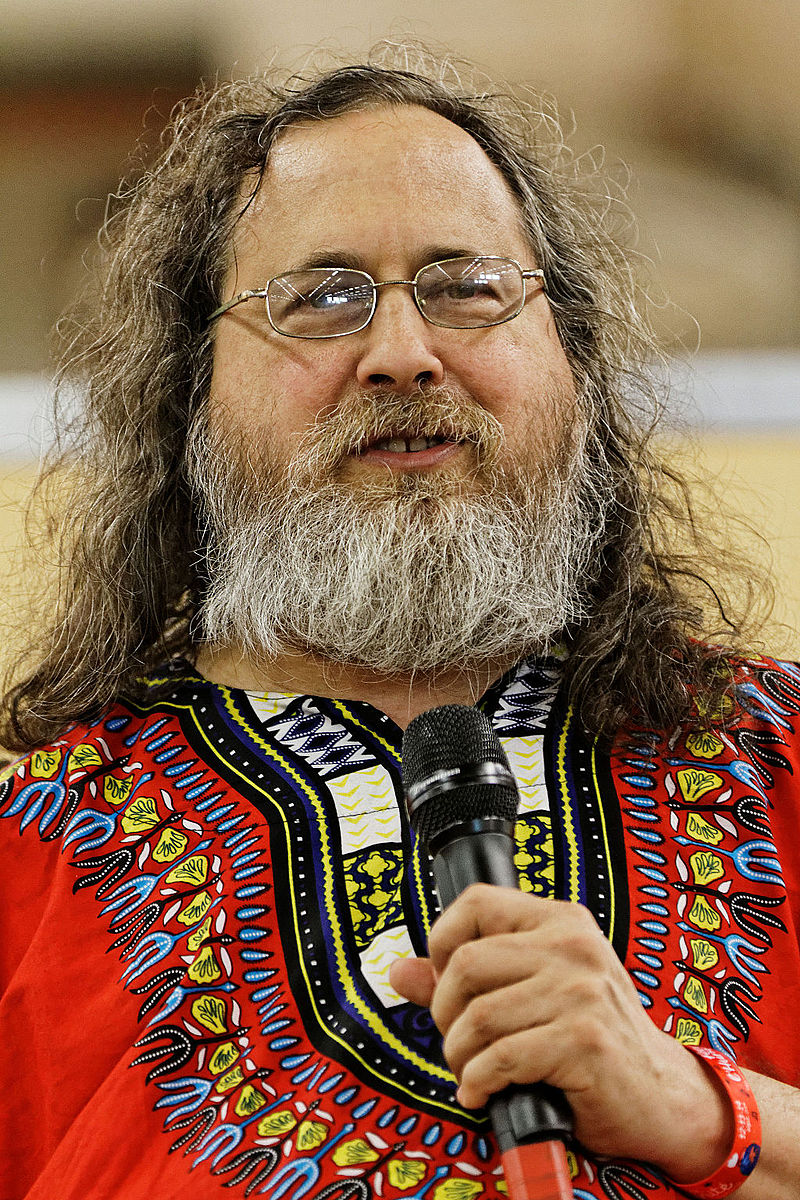
\includegraphics[width=\linewidth]{images/rms.jpg}
    \end{minipage}
    \hfill
    \begin{minipage}{0.45\textwidth}
        \centering
        
\includegraphics[width=\linewidth]{images/milei.jpg}
    \end{minipage}
\end{frame}


\begin{frame}{La libertad de Richard Stallman}
  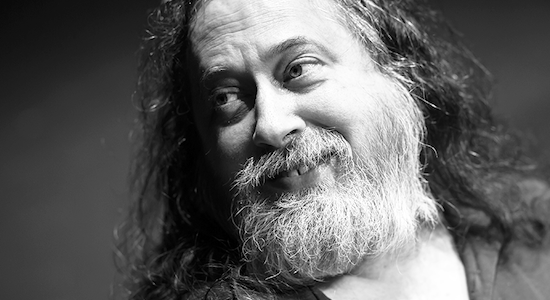
\includegraphics[width=\linewidth]{images/stallman.png}
\end{frame}

\begin{frame}{La libertad de Richard Stallman}
  \begin{itemize}
    \item Para Stallman, es la capacidad de controlar la tecnología que utilizamos. Es un concepto ético y moral, no solo técnico. \pause
  \item El software libre es cuestión de libertad, no de precio. Para entender
    el concepto, debes pensar en libertad como en 'libertad de expresión', no
    como en 'cerveza gratis'.
  \end{itemize}
\end{frame}

\begin{frame}{Las 4 Libertades de Richard Stallman}
  \begin{itemize}
    \item Libertad 0: Ejecutar el software con cualquier proósito \pause
    \item Libertad 1: Estudiar como funciona un programa de software y
      modificarlo segun sus necesidades. \pause
    \item Libertad 2: Redistribuir copias para ayudar a otros \pause
    \item Libertad 3: Distribuir versiones modificada, de modo que toda la
      comunidad se beneficie.
  \end{itemize}
\end{frame}

\begin{frame}{Implicaciones sociales del software libre}
\begin{itemize}
  \item Descentralización del poder, el software libre empodera a los usuarios,
    y les da el control sobre las herramientas que utilizan en su vida
    cotidiana. \pause
  \item Colaboración abierta, El modelo de desarrollo colaborativo del software
    libre sirve de inspiración para otras áreas, promoviendo comunidades basadas
    en el intercambio de conocimientos. \pause
  \item Ética y justicia, usar el software privativo, según Richard Stallman, es
    injusto por que limita la libertad de las personas. La ética debe prevalecer
    sobre el pragmatismo del uso de la tecnología.
\end{itemize}
\end{frame}


\begin{frame}{El impacto de las ideas del Software Libre en la sociedad}
  
\includegraphics[width=\linewidth]{images/amor.jpg}
\end{frame}

\begin{frame}{El impacto de las ideas del Software Libre en la sociedad}
  \begin{itemize}
    \item Transparencia y democracia, la filosofía del software libre se ha
      extendido  a otras áreas, como la ciencia abierta y los recursos
      educativos libres. \pause
    \item Modelos colaborativos, Wikipedia, Creative Commons, son ejemplos de
      cómo la filosofía del software libre  ha inspirado movimientos en el área
      del conocimiento y la cultura. \pause
    \item Para una sociedad más justa, los ciudadanos deben tener control total
      sobre las tecnologías que influyen en sus vidas, evitando que los
      gobiernos y las empresas restrinjan su libertad.
  \end{itemize}
\end{frame}

\begin{frame}{La filosofía del Software Libre en la vida cotidiana}
  \begin{itemize}
    \item Privacidad, usar software libre reduce la dependencia de tecnologías propietarias
      que pueden rastrear a los usuarios. \pause
    \item Educación, permiten a los estudiantes aprender sobre tecnología de
      forma libre y accesible, fomentando el conocimiento abierto. Y sin atarlos
      a ninguna tecnología o software en particular. \pause
    \item Economía, los modelos de negocio basados en servicio alrededor del
      software libre permiten el desarrollo económico sin sacrificar la libertad.
  \end{itemize}
\end{frame}

\begin{frame}
  Any powerful entity can take away people's freedom. That includes states and
  it includes businesses. Thus, the purpose of democracy is to use the state to
  protect us from businesses, while imposing limits on the state so that it does
  not become a tyranny.
  \vfill
  We are having great trouble defending the US against right-wing
  conspirancies, headed by billionaires in leage with Trump and using
  anti-social media to spread disinformation.
\end{frame}

\begin{frame}
  \centering
  \Huge Esto tiene buena pinta, pero...
\end{frame}

\begin{frame}{La libertad según Javier Milei}
  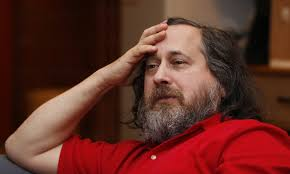
\includegraphics[width=\linewidth]{images/uyy.jpeg}
\end{frame}

\begin{frame}{La libertad según Javier Milei}
    \begin{itemize}
        \item Javier Milei se autodenomina "liberal libertario". \pause
        \item Defiende la libertad económica y rechaza la intervención estatal. \pause
        \item La libertad, para Milei, es la capacidad de cada individuo de
          decidir sin restricciones del Estado. \pause
        \item Crítica las políticas que limitan el mercado.
    \end{itemize}
\end{frame}

\begin{frame}
    \centering
    \Huge ¿Qué es la libertad?
\end{frame}
\end{document}
